% MIT License

% Copyright (c) 2022 Chiyuru

% Permission is hereby granted, free of charge, to any person obtaining a copy of this software and associated documentation files (the "Software"), 
% to deal in the Software without restriction, including without limitation the rights
% to use, copy, modify, merge, publish, distribute, sublicense, and/or sell
% copies of the Software, and to permit persons to whom the Software is
% furnished to do so, subject to the following conditions:

% The above copyright notice and this permission notice shall be included in all copies or substantial portions of the Software.

% THE SOFTWARE IS PROVIDED "AS IS", WITHOUT WARRANTY OF ANY KIND, EXPRESS OR IMPLIED, INCLUDING BUT NOT LIMITED TO THE WARRANTIES OF MERCHANTABILITY,
% FITNESS FOR A PARTICULAR PURPOSE AND NONINFRINGEMENT. IN NO EVENT SHALL THE AUTHORS OR COPYRIGHT HOLDERS BE LIABLE FOR ANY CLAIM, DAMAGES OR OTHER
% LIABILITY, WHETHER IN AN ACTION OF CONTRACT, TORT OR OTHERWISE, ARISING FROM,
% OUT OF OR IN CONNECTION WITH THE SOFTWARE OR THE USE OR OTHER DEALINGS IN THE SOFTWARE.

\documentclass[UTF8]{ctexart}

\usepackage{amssymb}
\usepackage{amsmath}
\usepackage{cases}
\usepackage{cite}
\usepackage{graphicx}
\usepackage[margin=1in]{geometry}
\geometry{a4paper}
\usepackage{fancyhdr}
\pagestyle{fancy}
\fancyhf{}


\title{作业三报告}
\author{
    刘锦坤
    \\2022013352}
\date{\today}
\pagenumbering{arabic}

\begin{document}

\fancyhead[C]{深度学习算法报告}
\fancyfoot[C]{\thepage}

\maketitle

\section{Question1}

\begin{figure}[h]
    \centering
    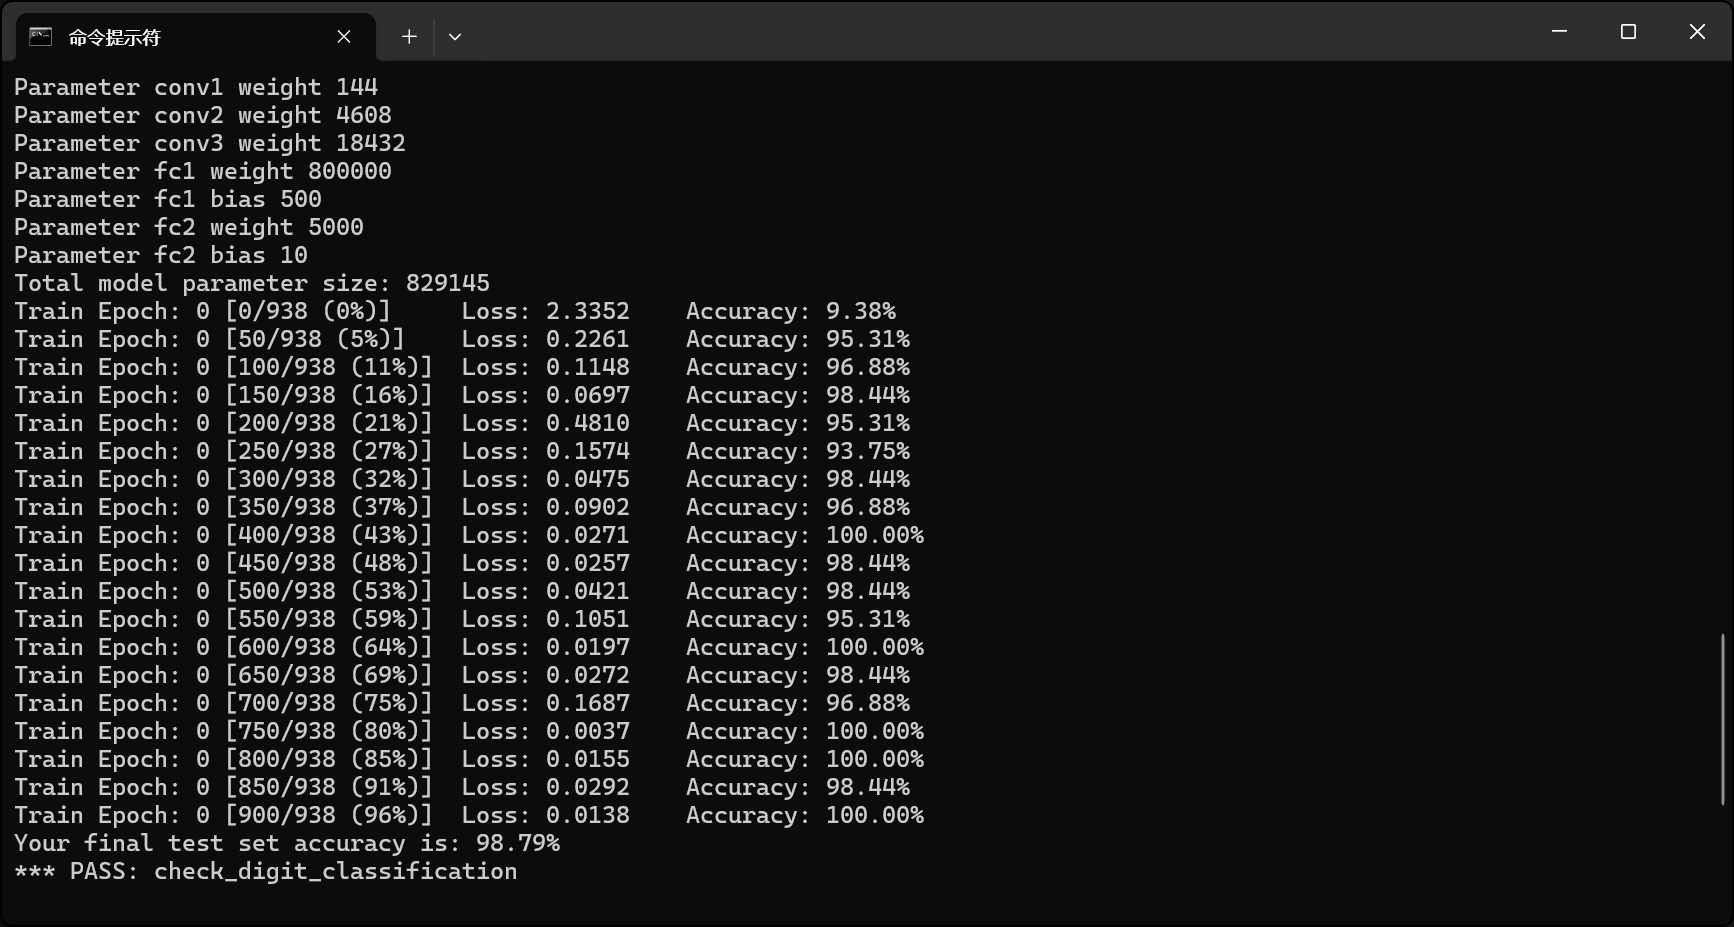
\includegraphics[width=0.8\textwidth]{./image/Batch.png}
    \caption{BatchNorm Layer}
    % 设置引用标签
    \label{fig:Batch}
\end{figure}

\begin{figure}[h]
    \centering
    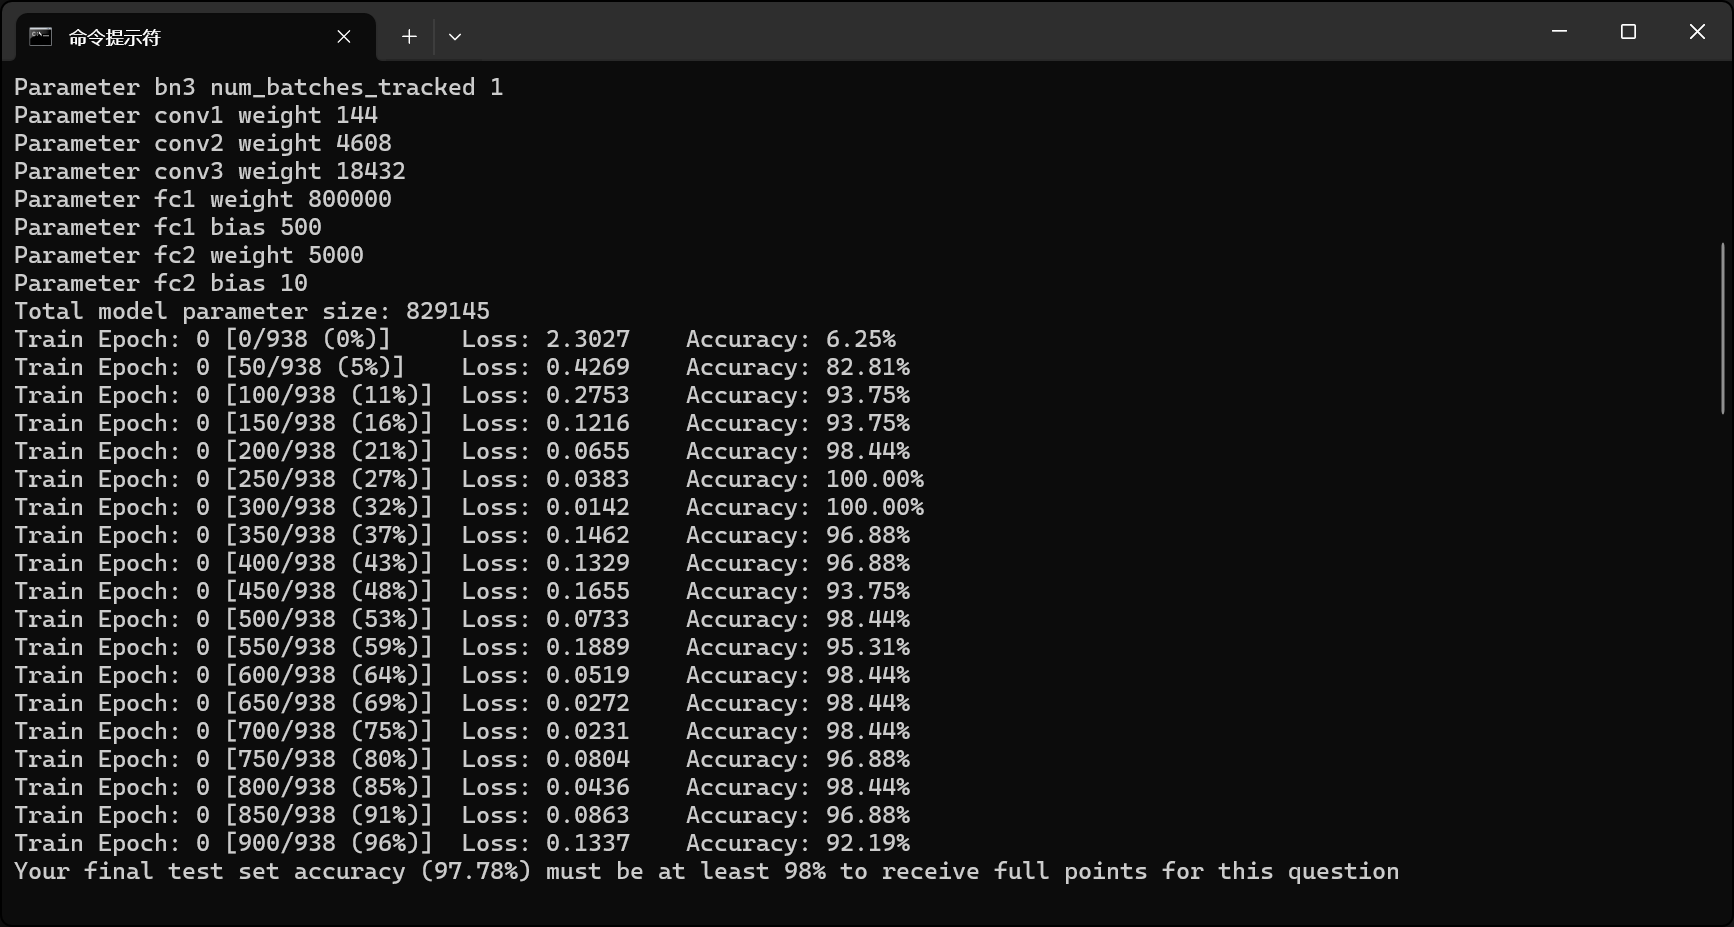
\includegraphics[width=0.8\textwidth]{./image/NoBatch.png}
    \caption{Without BatchNorm Layer}
    % 设置引用标签
    \label{fig:NoBatch}
\end{figure}

BatchNorm Layer的重要作用是加速模型的收敛,BatchNorm Layer将每个批量内的数据都进行了标准化处理,从而减少了由于前面的层输入参数变化导致的偏移量,进而使得模型收敛更迅速。

图\ref{fig:Batch}是加入BatchNorm Layer的模型,图\ref{fig:NoBatch}是没有加入BatchNorm Layer的模型,可以看到加入BatchNorm Layer的模型收敛速度更快,而且收敛到的结果更好。

\section{Question2}

图\ref{fig:Adversarial}展示了生成的对抗性样本,可以做如下分析:

根据FGSM的原理,对抗样本在原始图像上添加了扰动,具体表现在一些像素强度上的改变,可能某些像素强度变高或者变低,或者像最左边那些数字一样整体像素强度都变得很低。

这些对抗性样本能够欺骗LeNet的原理大致可以归于以下:

\begin{enumerate}
    \item 通过反向的“梯度上升”,找到使得损失函数最大化的方向,从而生成对抗性样本,欺骗了模型。
    \item 但是这也说明的LeNet Model本身对于微扰是非常敏感的,即使微小的变化也能通过网络层传播并放大,从而导致输出发生显著变化。
    \item 但是最后的对抗性样例不能欺骗人眼,就说明这是LeNet泛化能力不足的体现,这些对抗样本事实上就利用了LeNet学习到的那些噪声特征进行欺骗。
\end{enumerate}
\begin{figure}[h]
    \centering
    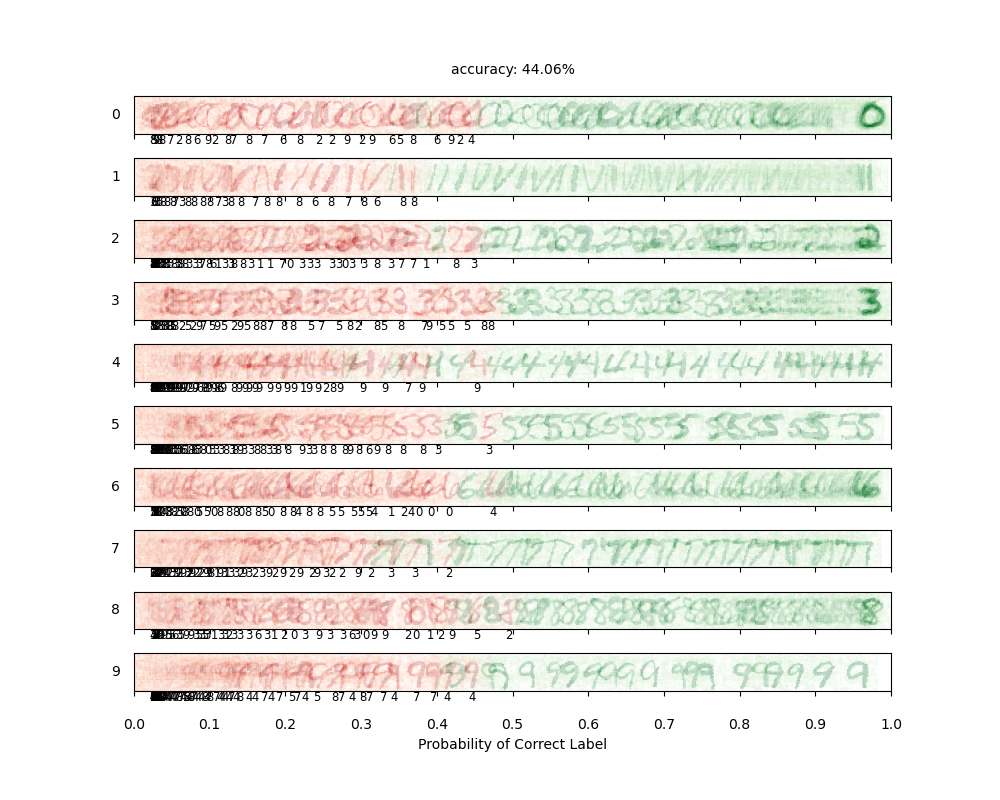
\includegraphics[width=0.8\textwidth]{./image/Adversarial.png}
    \caption{Adversarial Example}
    % 设置引用标签
    \label{fig:Adversarial}
\end{figure}

\section{算法分析}

Here is the modified code:

\section{算法分析}

这里对于本次作业中使用到的各个方法进行一个简要的分析:

\subsection{Task1}

这一部分主要使用CNN Layer, BatchNorm Layer, ReLU, Pool Layer, FullConnected Layer等方法进行手写数字集的识别,卷积层主要是对图像中的各个模态进行识别,批归一化层用以加速收敛和提高泛化能力,池化层将数据模糊化,也起到提高泛化能力的作用,最后利用全连接层作为感知机,对于前面提取到的特征进行分类。

\subsection{Task2}

这一部分就是用全连接层做一个函数图像的拟合,事实上存在神经网络的任意逼近定理,大致即为一个包含足够多隐含层神经元的多层前馈网络,能以任意精度逼近任意预定的连续函数,而这里的回归结果可以看成这个定理的一个体现。\footnote{参考https://blog.csdn.net/qq\_37983752/article/details/115055707}
\subsection{Task3}

这一部分内容在于对抗性样本的生成,这里使用了FGSM方法,即通过对原始图像添加一个扰动,使得模型的损失函数最大化,从而生成对抗性样本,这里的对抗性样本实际上就是利用了模型的一些特性,通过微扰来欺骗模型。

\subsection{Task4}

这一问使用RNN对于文本的语言进行了分类,RNN是一种针对序列输入提出的神经网络,将状态和特征在序列的元素之间传递最终输出,这种方法的优势在于能够处理序列数据,比如文本,时间序列等,在面对序列数据时可以用较少的参数完成较好的提取特征。
\end{document} 